\section{Mediciones y resultados obtenidos}

Para la implementación del circuito se buscó en las simulaciones tener una ganancia de corriente mayor a 60 veces, una ganancia de tensión mayor a 80\%, siempre cuidando que ambos transistores queden correctamente polarizados, teniendo en cuenta que uno tiende a la saturación y el otro al corte. De esa forma se llegó a los valores dados de los componentes. En la Figura \ref{circ_proto} se muestra la implementación del circuito en protoboard.

		\begin{figure}[H]
			\centering
			\resizebox{0.7\textwidth}{!} {%
				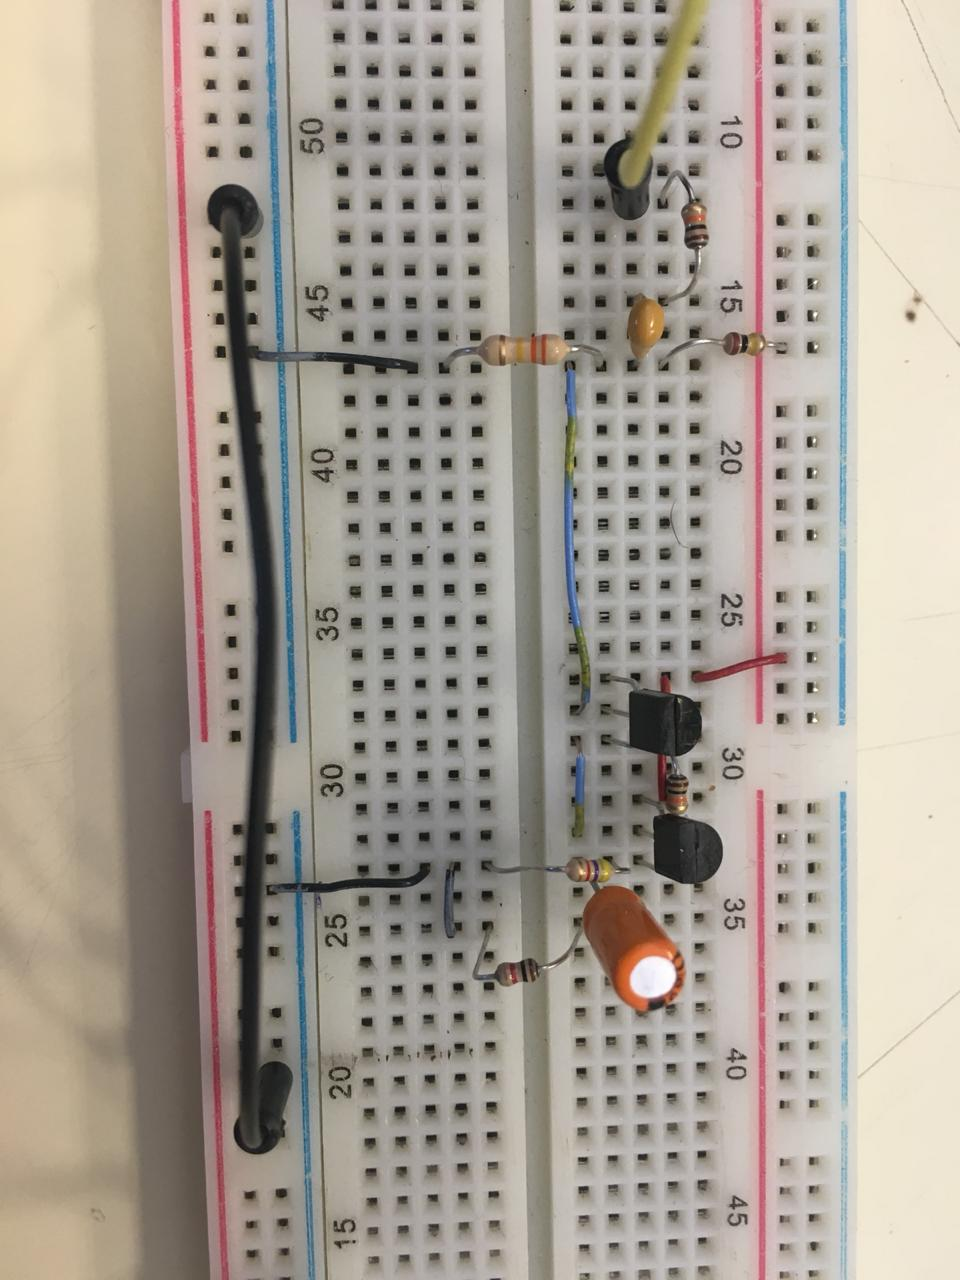
\includegraphics[angle=90]{./Imagenes/circuito_proto.jpeg} 
			}
			\caption{Circuito armado en protoboard.}
			\label{circ_proto}
		\end{figure}

\subsection{Polarización}
La comparación entre los valores de la polarización de los transistores se muestran en la Tabla\ref{tabla_polarizacion_comp}. Las diferencias en las $I_{CQ}$ se deben principalmente a las variaciones de $\beta$ con $I_{C}$, que fueron tenidas en consideración en los cálculos teóricos, pero de todas formas es distinto al real.

	\begin{table}[h!]
		\centering
		\begin{tabular}{c c c c}%
			\bfseries &Te\'orico & Medido & Simulado \\ \hline \\
			$V_{CEQ1} (V)$ & $4,01$ &$4,00$ & $4,03$ \\
			$V_{CEQ2} (V)$ & $4,71$& $4,60$& $4,64$\\
			$I_{CQ1} (\mu A)$ & $93,54$&$66$ & $66,5$\\
			$I_{CQ2} (mA)$ &$2,30$ & $2,10$& $2,1$\\
			$V_{BE1} (V)$ &$0,7$ &$0,52$ & $0,53$\\
			$V_{BE2} (V)$ & $0,7$& $0,6$& $0,61$\\
			\hline
		\end{tabular}
		\caption{Comparaci\'on de valores de polarizaci\'on para los casos te\'orico, medido y simulado.}
		\label{tabla_polarizacion_comp}
	\end{table}

\subsection{Ganancias}
En primer lugar, se midió la ganancia de tensión del sistema. En la Figura \ref{fig_bode_avs} se muestra la contrastación de la medición, la simulación y la teoría. Como ningún cálculo teórico tiene en cuenta variaciones con la frecuencia, se toma un único valor para todas las frecuencias, y se ve que la aproximación para frecuencias medias es válida en el intervalo de frecuencias entre 400$Hz$ y 500$kHz$, donde la ganancia empieza a caer. La ganancia en la banda pasante simulada a 1$kHz$ es de 0.869 veces y la medida es de 0.863 veces, con lo que el cálculo teórico de 0.866 veces resulta muy cercano a la realidad.

	\begin{figure}[H]
		\centering
		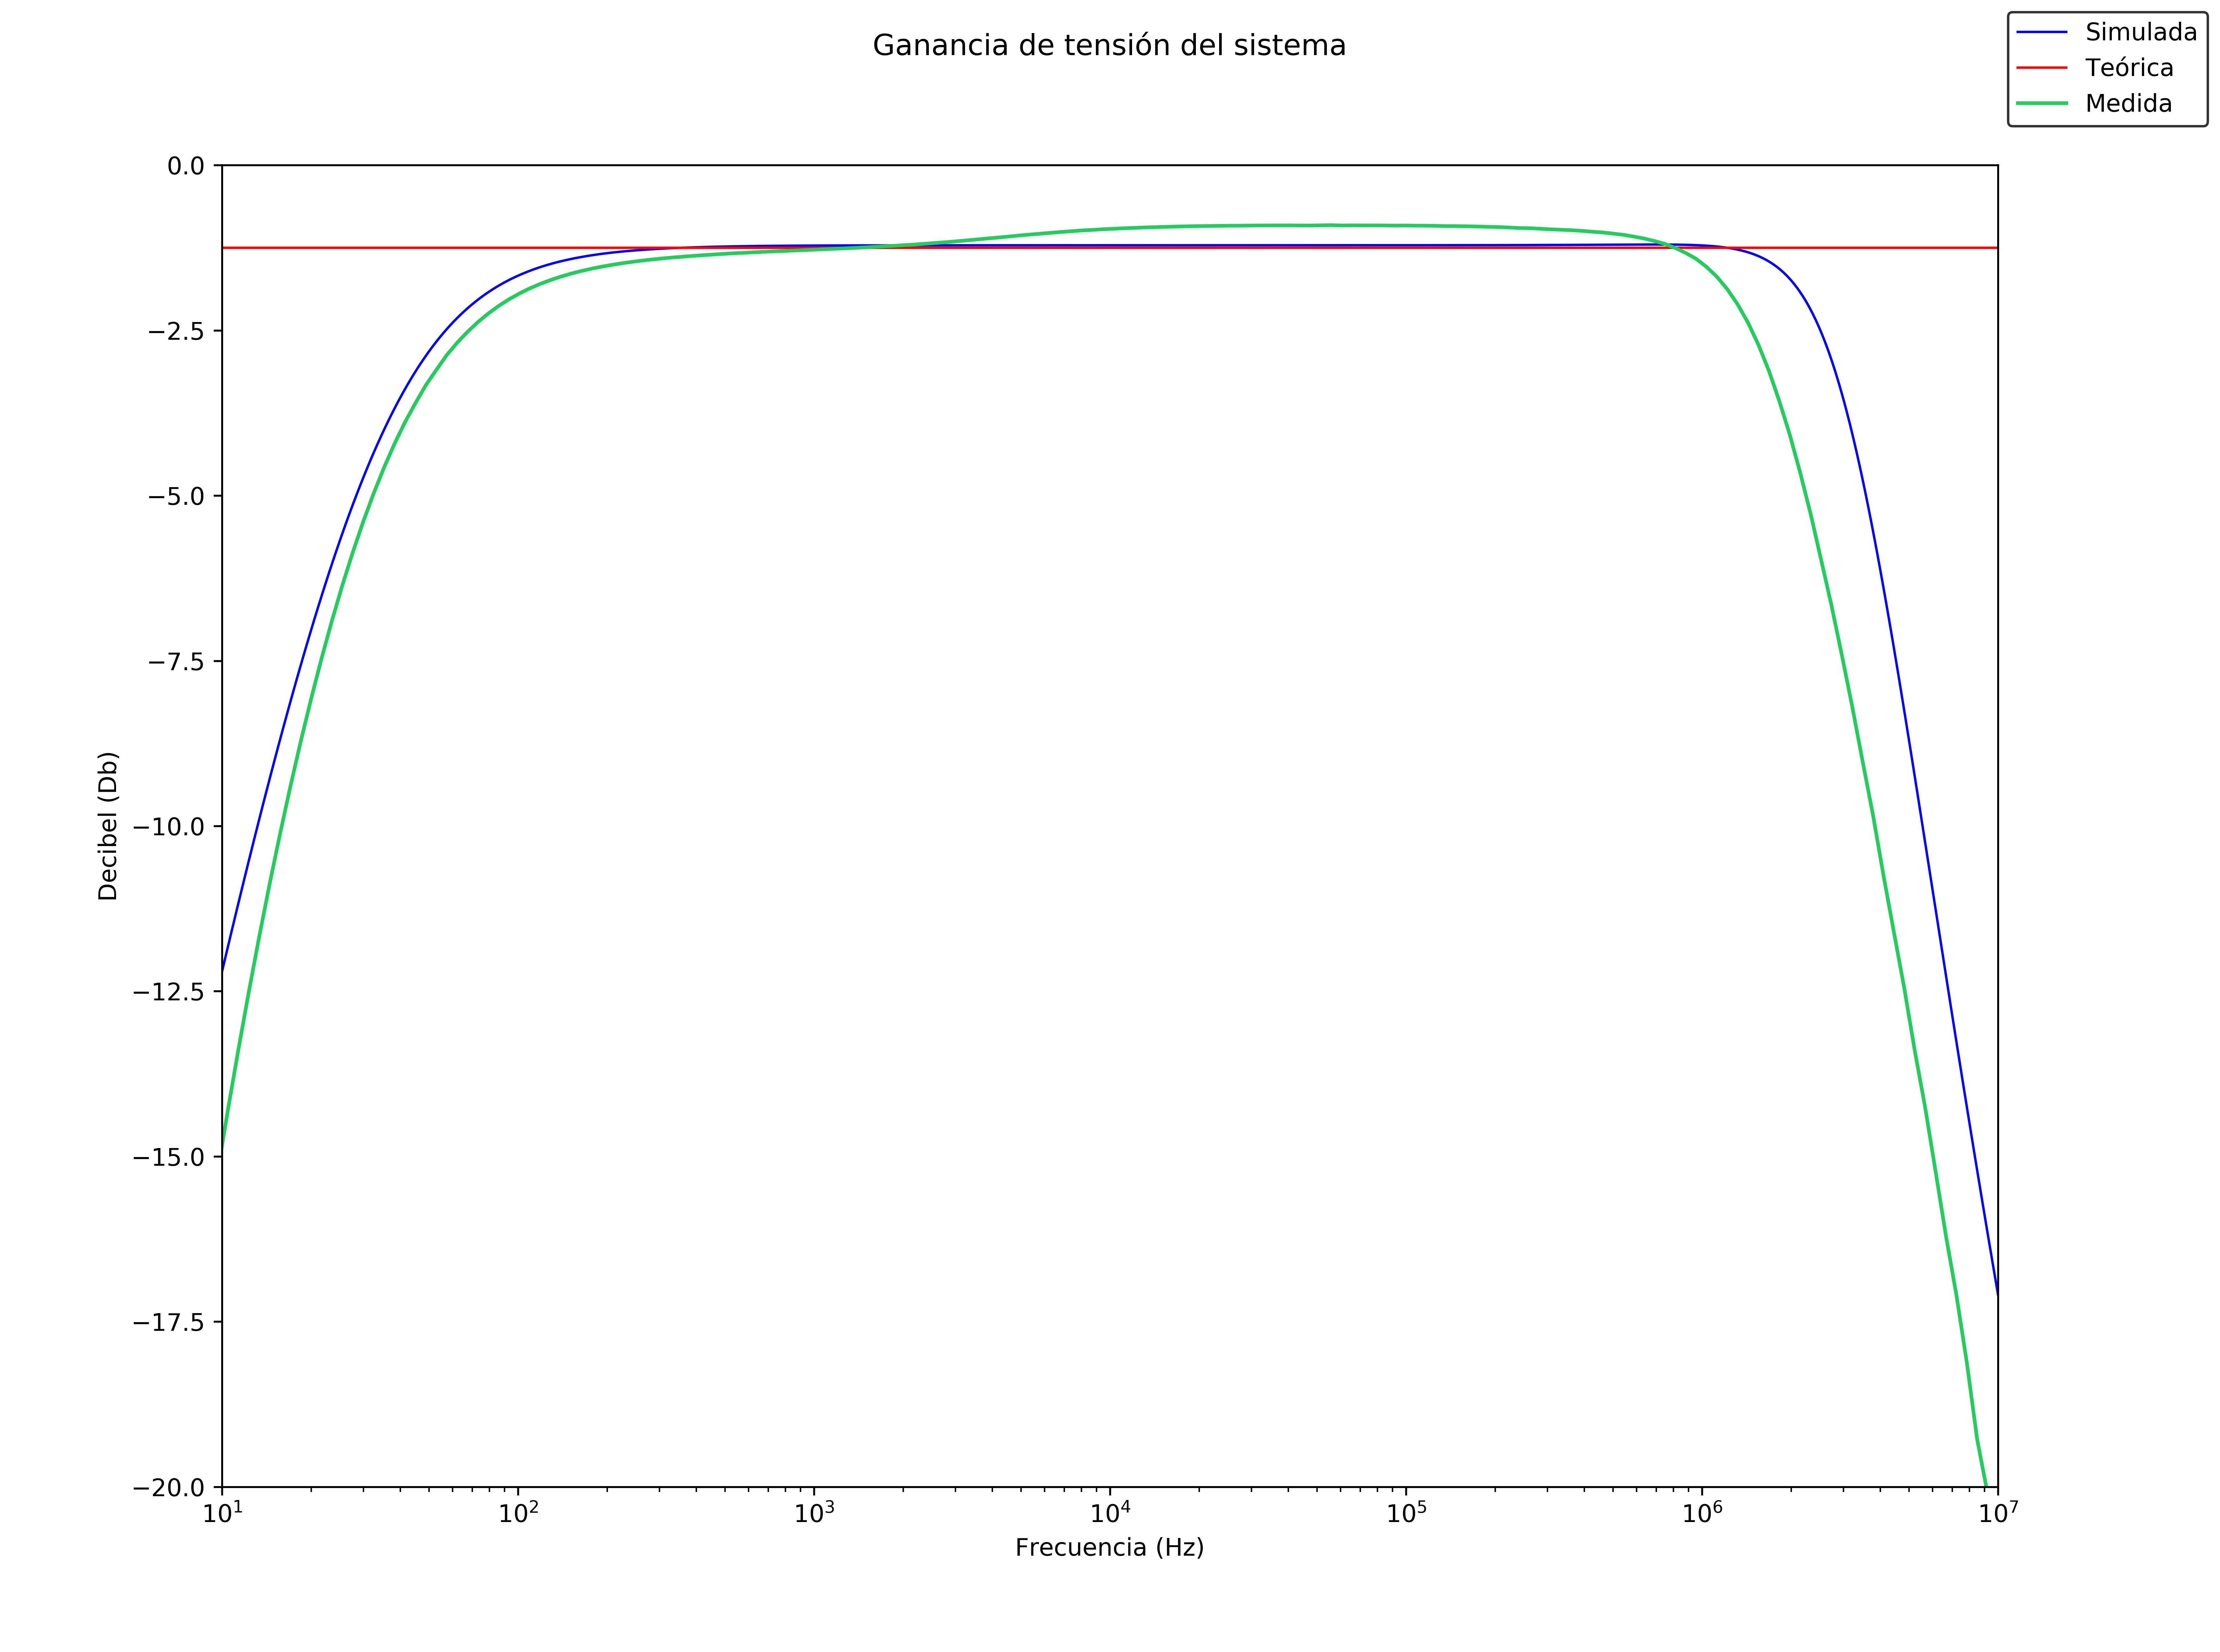
\includegraphics[scale=0.4]{./Imagenes/bode_Avs.png} \\
		\caption{Ganancia de tensión del sistema teórica, simulada y medida}
		\label{fig_bode_avs}
	\end{figure}

Luego se midió la ganancia de corriente del sistema. En la Figura \ref{fig_bode_ais} se puede observar la comparación entre teoría, simulación y práctica. En éste caso, es menor el intervalo de frecuencias en las que es válida la estimación teórica, y se presenta una diferencia entre simulación y medición en el punto en el que empieza a caer la ganancia. Éste efecto puede ser atribuible a las capacidades introducidas por el protobard. A $1kHz$, la ganancia en la banda pasante simulada es de 37.541 dB, 75.34 veces, la medida de 37.587 dB, 75.74 veces, mientras que la teórica es de 74 veces, con lo que el modelo nuevamente se verifica. 

	\begin{figure}[H]
		\centering
		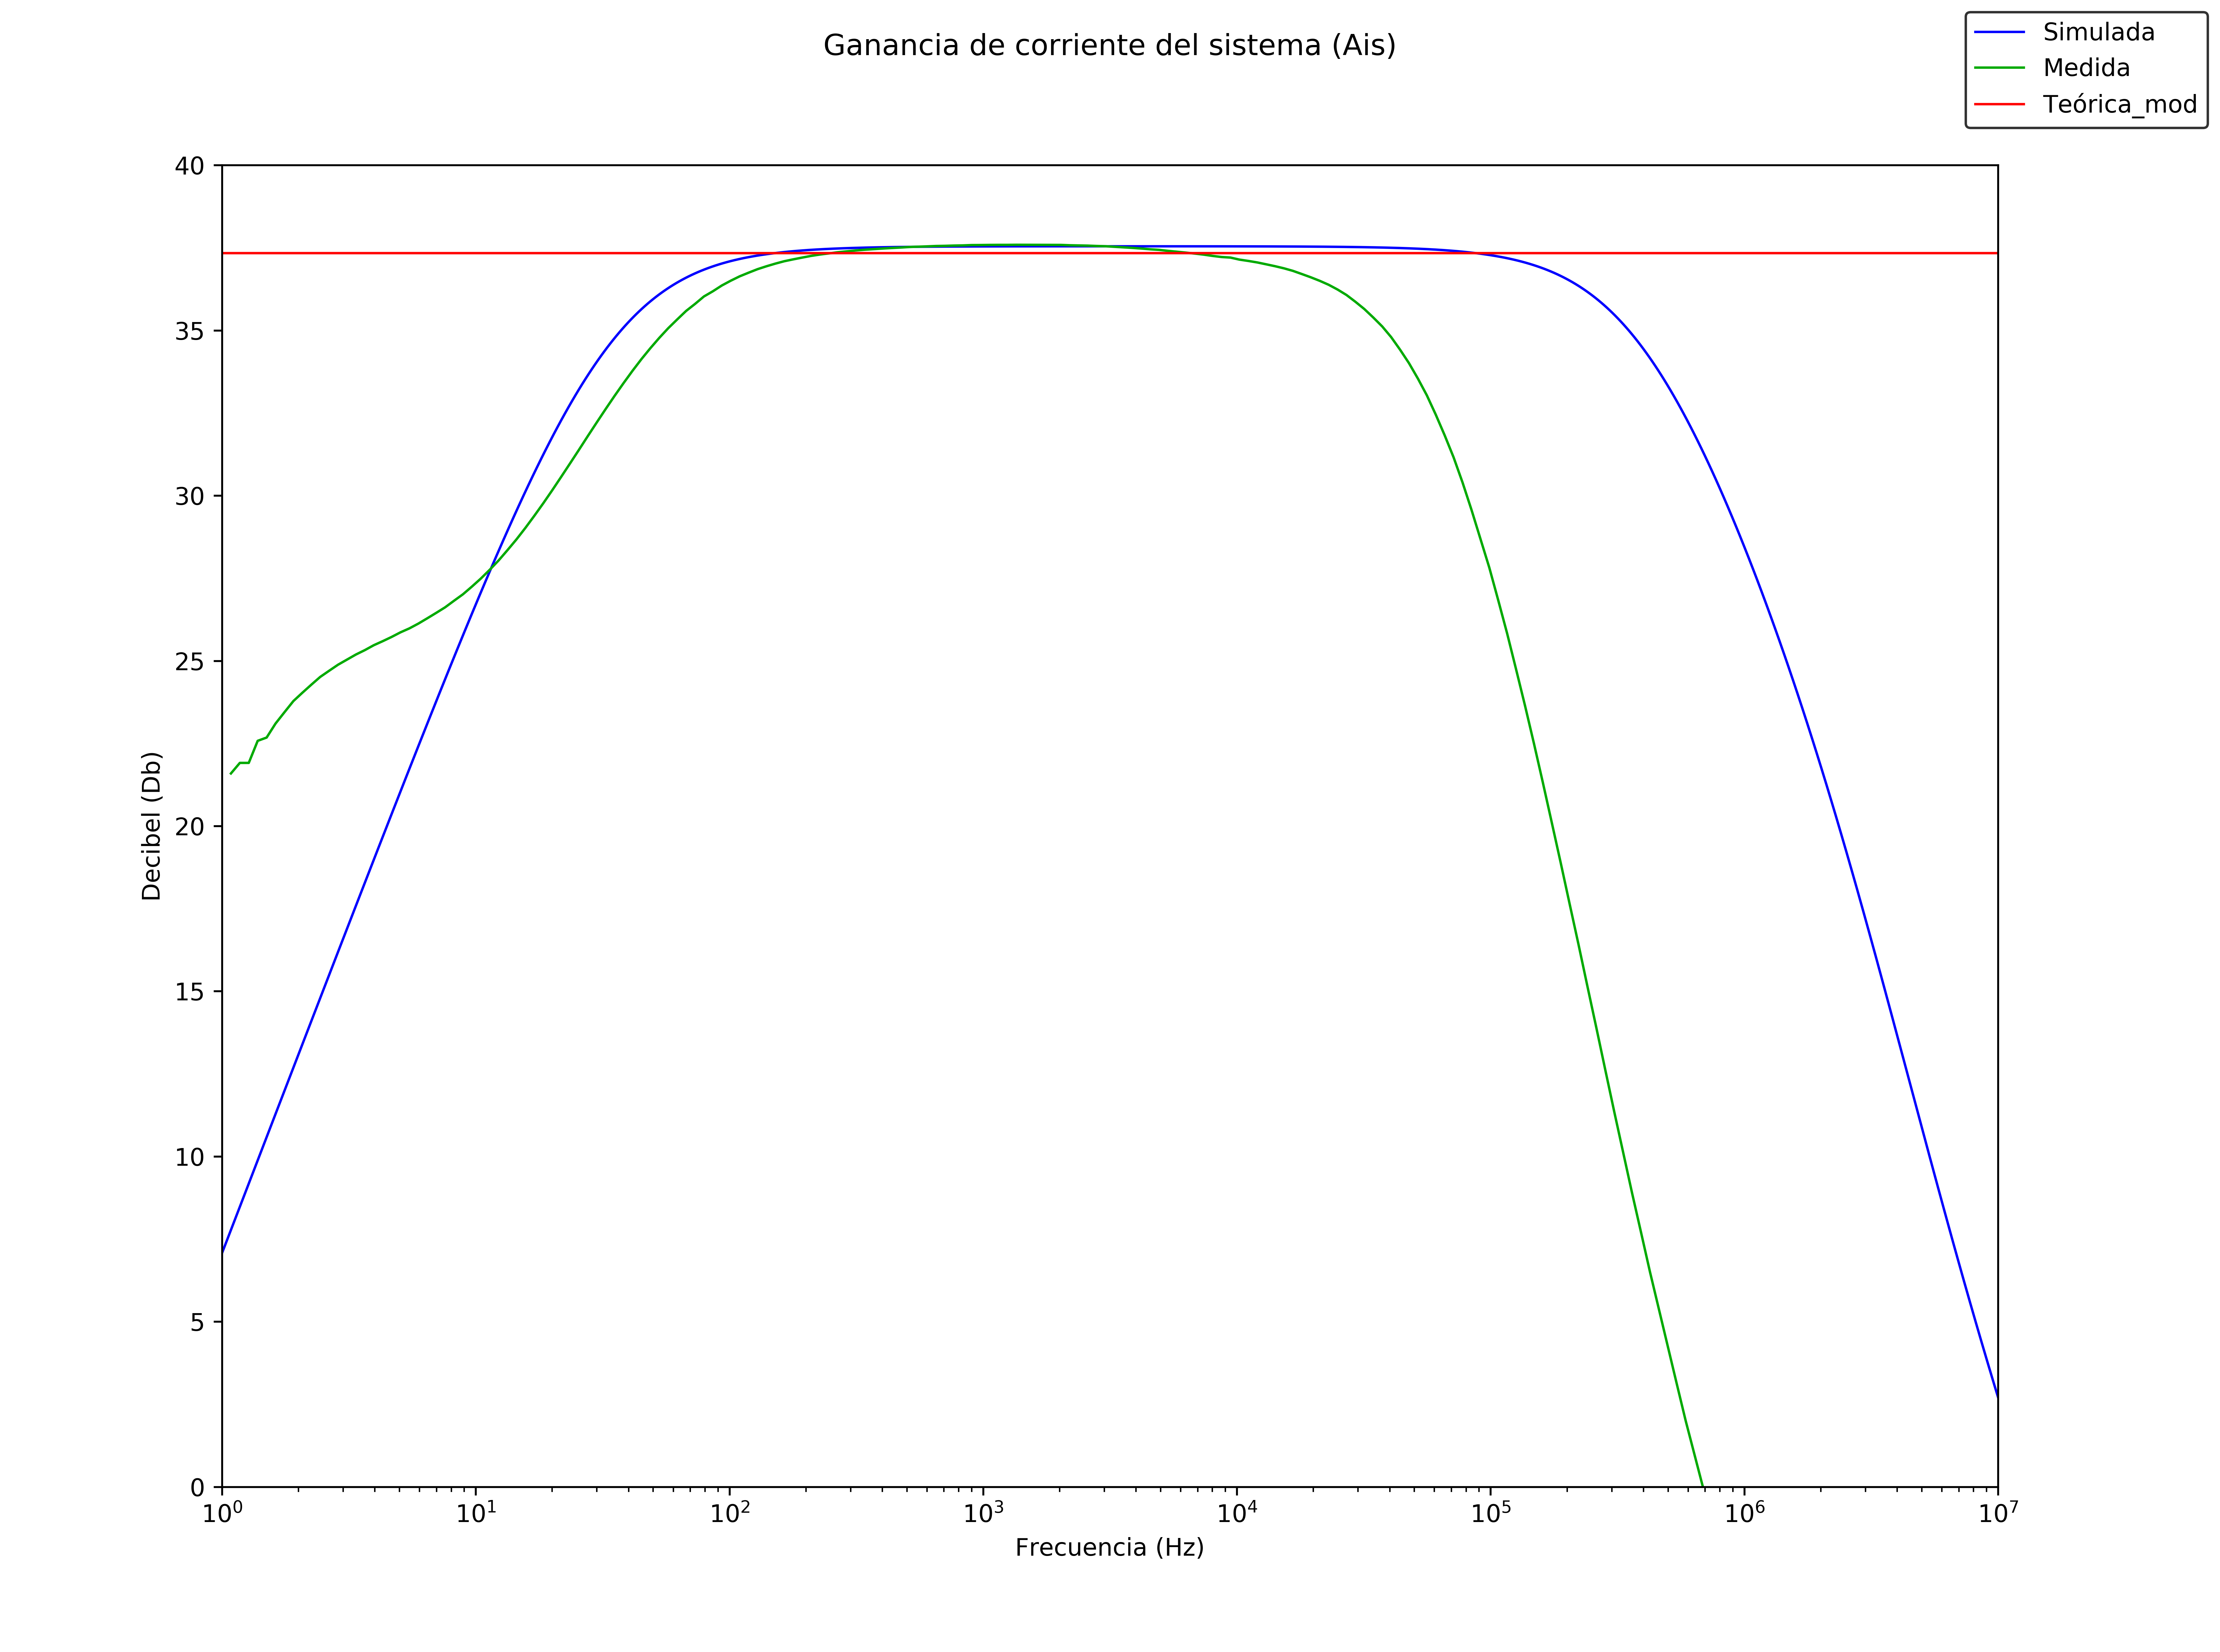
\includegraphics[scale=0.3]{./Imagenes/bode_Ais.png} \\
		\caption{Ganancia de corriente del sistema teórica, simulada y medida}
		\label{fig_bode_ais}
	\end{figure}

\subsection{Impedancias}
Con respecto a la impedancia de entrada, se muestra la contrastación entre teoría, simulación y medición en la Figura \ref{fig_bode_zin}, donde se puede apreciar que para frecuencias inferiores a 10$kHz$ las tres curvas son cercanas, siendo la impedancia de entrada medida a 
$1kHz$ $85k\Omega$, mientras que la simulada a la misma frecuencia es de $86,66 k\Omega$, y la teórica es de $85k\Omega$. Se observa que la impedancia de entrada a bajas frecuencias es muy alta, ésto se debe al capacitor que hay en la entrada. 

	\begin{figure}[H]
		\centering
		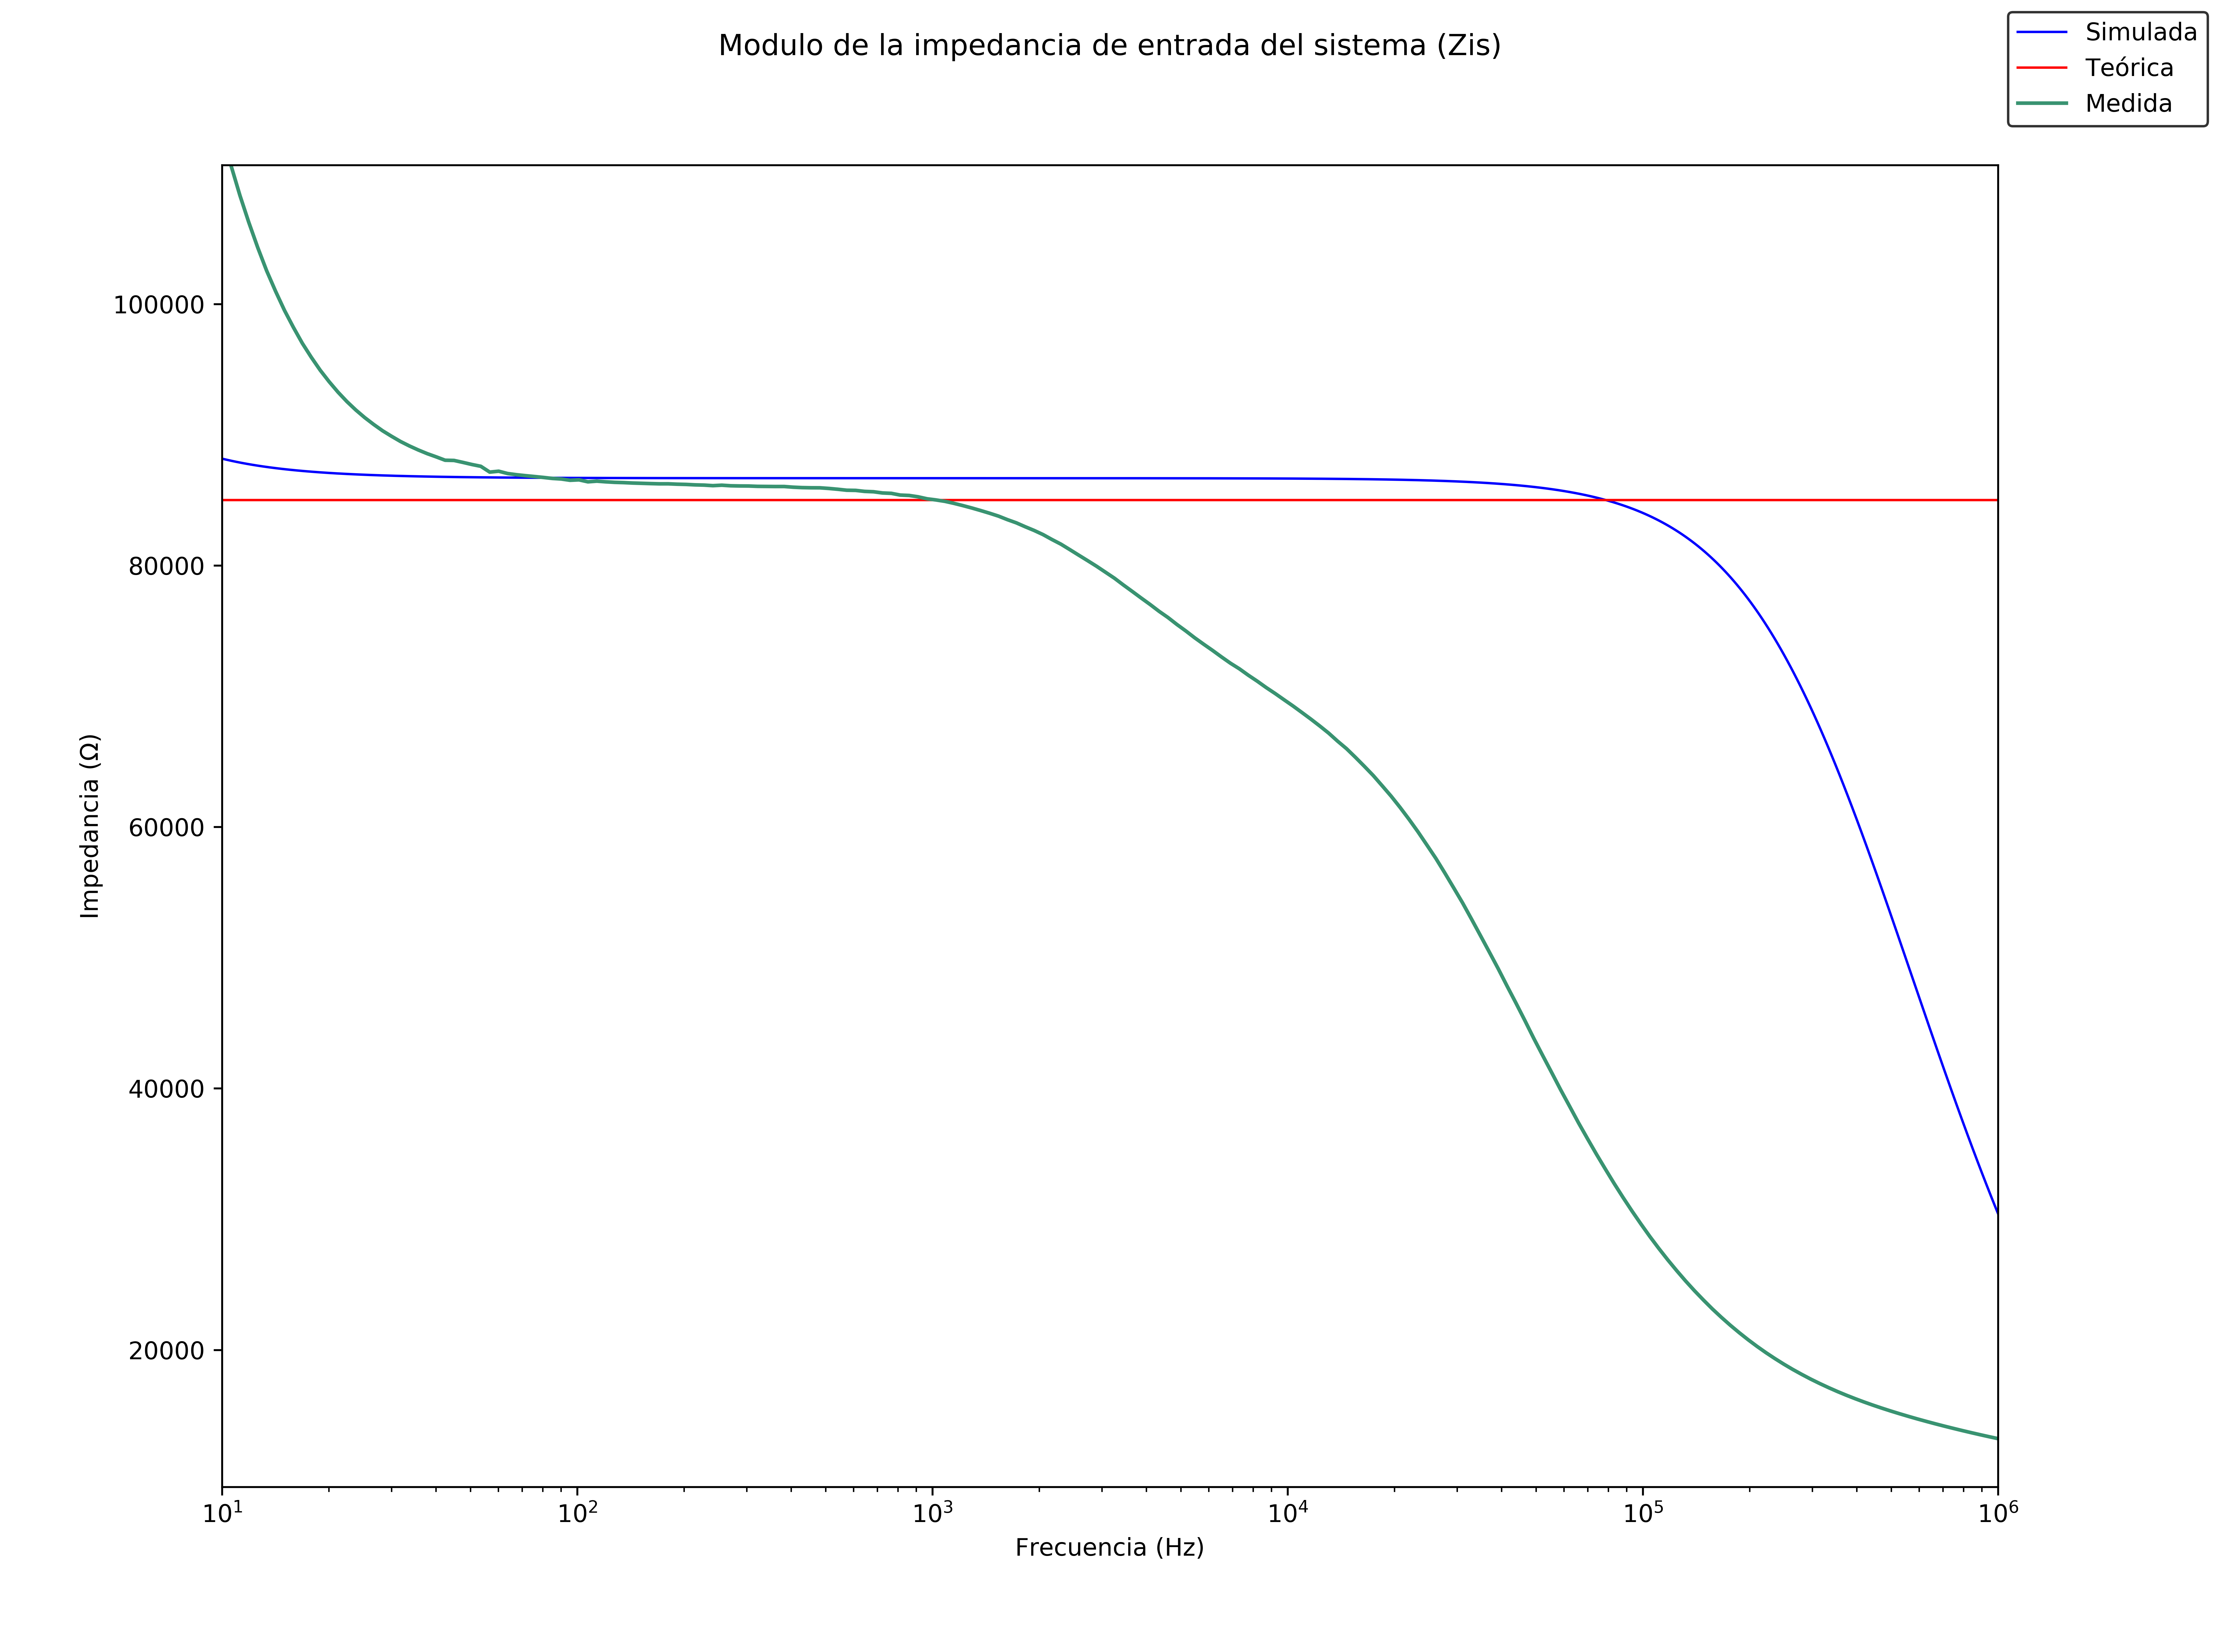
\includegraphics[scale=0.4]{./Imagenes/Modulo_zin.png} \\
		\caption{Impedancia de entrada del sistema teórica, simulada y medida.}
		\label{fig_bode_zin}
	\end{figure}

Para la impedancia de salida se muestra la contrastación entre teoría, simulación y práctica en la Figura \ref{fig_bode_zout}. Se observa que el sistema presenta una baja impedancia de salida, lo cual era esperado por tratarse de un colector común. A $1kHz$, la impedancia medida es de 32.97$\Omega$, la simulada es de 35.89$\Omega$ y la teórica es de 17,52$\Omega$. Sin embargo, se observa que a partir de 3$kHz$, que también puede ser considerado una frecuencia media, hay una mayor correspondencia entre simulación, medición y teoría.

		\begin{figure}[H]
			\centering
			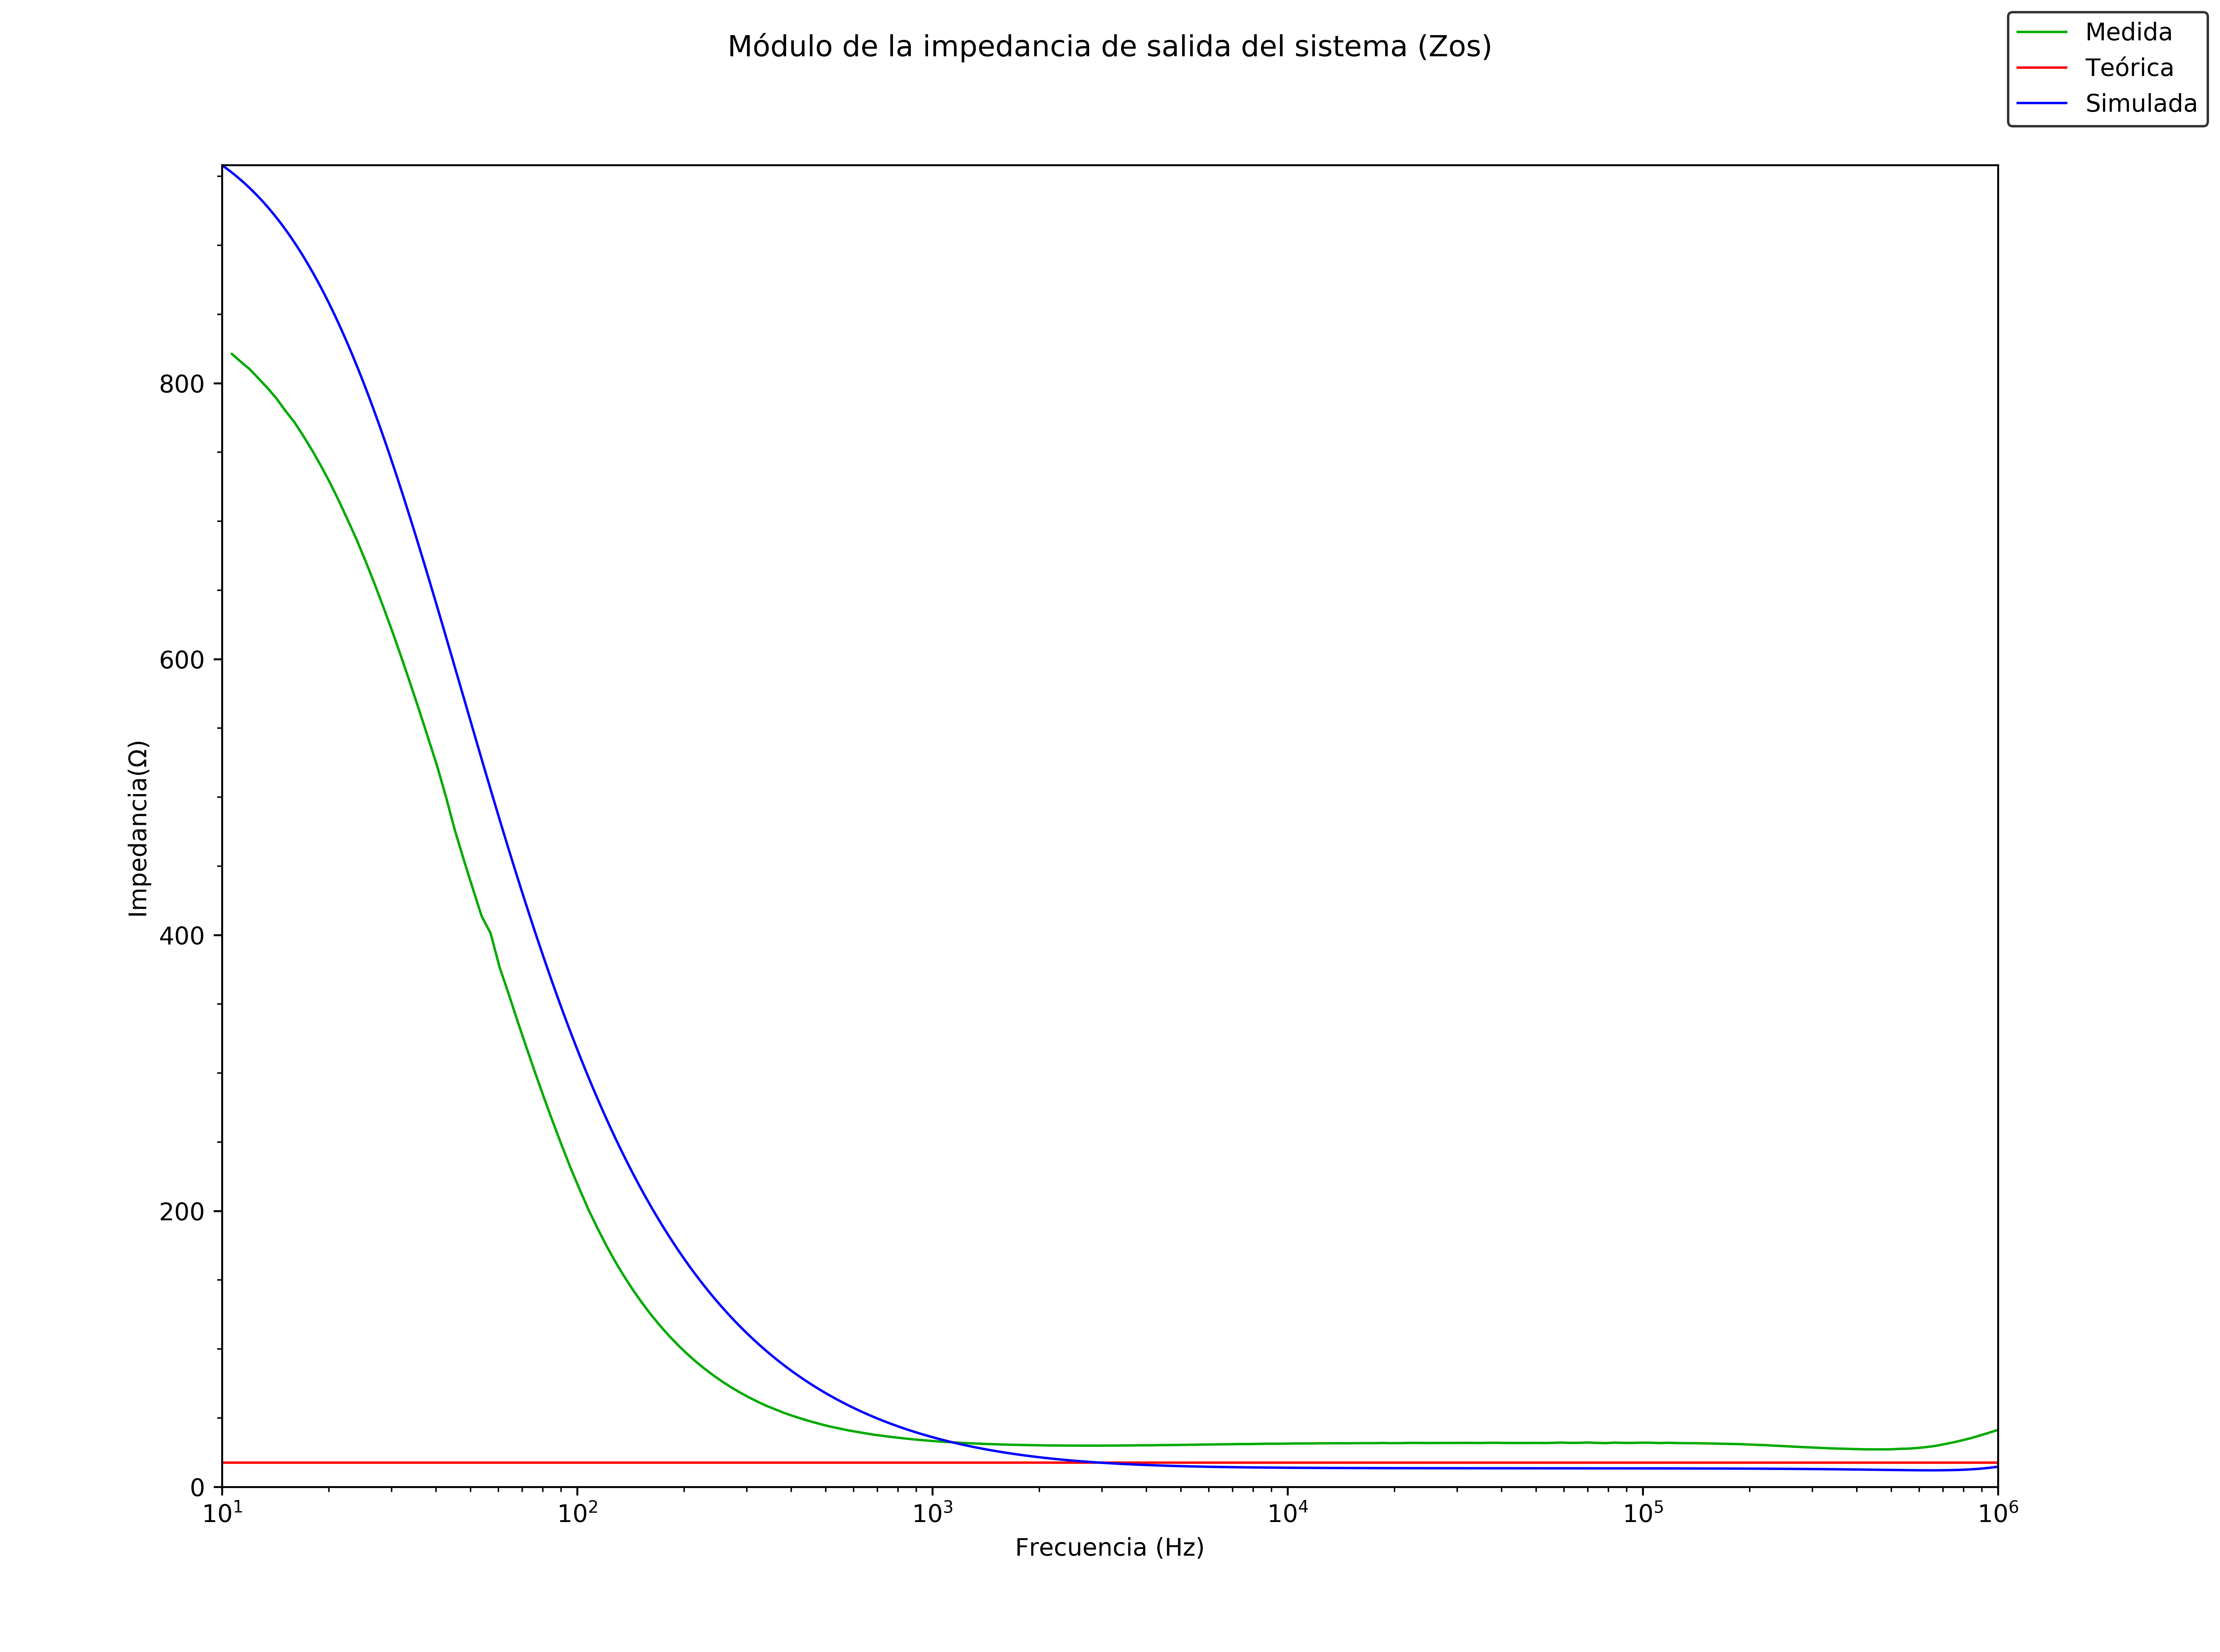
\includegraphics[scale=0.4]{./Imagenes/Modulo_zos.png} \\
			\caption{Impedancia de salida del sistema teórica, simulada y medida.}
			\label{fig_bode_zout}
		\end{figure}
 
\subsection{Resumen}

En la Tabla \label{valores_frec_media} se muestran los valores teóricos, simulados y medidos de las ganancias e impedancias para $1kHz$, frecuencia media.

	\begin{table}[H]
		\centering
		\begin{tabular}{c c c c }
					%\begin{tabular}{|c|c|c|c|}
		\hline
		Parámetro   	   & Teórico & Simulado & Medido \\ \hline
		$\Delta _{VS} (veces)$ 	   & 0,87    & 0,87     & 0,86   \\% \hline
		$\Delta_{IS} (veces)$	   & 74      & 75,74    & 75,34  \\ %\hline
		Zis ($k\Omega$)  & 85      & 86,66    & 85     \\ %\hline
		Zos  ($\Omega$) & 17,52   & 35,89    & 32,97  \\ \hline
		\end{tabular}
		\caption{Valores teóricos, simulados y medidos de los distintos parámetros a frecuencias medias.}
		\label{valores_frec_media}
	\end{table}
